\chapter[Continuous Deep Equilibrium Networks]{Continuous Deep Equilibrium Networks: Training Neural ODEs Faster by Integrating Them to Infinity}
\label{chapter:infinite_time_neural_odes}

Implicit layer methods, such as Neural ODEs and Deep Equilibrium models~\citep{chen2018neural, bai_deep_2019, ghaoui_implicit_2020}, have gained popularity due to their ability to automatically adapt model depth based on the ``complexity'' of new problems and inputs. The forward pass of these methods involves solving steady-state problems, convex optimization problems, differential equations, etc., all defined by neural networks, which can be expensive. However, training these more generalized models has empirically been shown to take significantly more time than traditional explicit models such as recurrent neural networks and transformers. \textit{Nothing within the problem's structure requires expensive training methods, so we asked, can we reformulate continuous implicit models so that this is not the case}?

\citet{grathwohl2018ffjord, dupont2019augmented, kelly2020learning, finlay2020train} have identified several problems with training implicit networks. These models grow in complexity as training progresses, and a single forward pass can take over 100 iterations~\citep{kelly2020learning} even for simple problems like MNIST. Deep Equilibrium Models~\citep{bai_deep_2019, bai_multiscale_2020} have better scaling in the backward pass but are still bottlenecked by slow steady-state convergence. \citet{bai2021stabilizing} quantified several convergence and stability problems with DEQs. They proposed a regularization technique by exploiting the ``implicitness" of DEQs to stabilize their training. \textit{We marry the idea of faster backward pass for DEQs and continuous modeling from Neural ODEs to create Infinite Time Neural ODEs which scale significantly better in the backward pass and drastically reduce the training time}. % However, such a regularization process is expensive as it requires higher-order automatic differentiation. Their results demonstrated faster prediction times at the expense of greatly increased training times. This leaves an open question as to whether such regularization could be imposed in a cheap or free enough manner to reduce the training cost.

Our main contributions include\footnote{Our code is publicly available at \url{https://github.com/SciML/DeepEquilibriumNetworks.jl}}:
%
\begin{enumerate}
  \item An improved DEQ architecture (Skip-DEQ) that uses an additional neural network to predict better initial conditions.

  \item A regularization scheme (Skip Regularized DEQ) incentivizes the DEQ to learn simpler dynamics and leads to faster training and prediction. Notably, this does not require nested automatic differentiation and thus is considerably less computationally expensive than other published techniques.

  \item A continuous formulation for DEQs as an infinite time neural ODE, which paradoxically accelerates the backward pass over standard neural ODEs by replacing the continuous adjoints with a simple linear system.

  \item We demonstrate the seamless combination of Continuous DEQs with Skip DEQs to create a drop-in replacement for Neural ODEs without incurring a high training cost.
\end{enumerate}
%

The contents of this chapter has appeared in the pre-print: Pal, A., Edelman, A. and Rackauckas, C., 2022. Continuous Deep Equilibrium Models: Training Neural ODEs Faster by Integrating Them to Infinity. arXiv preprint arXiv:2201.12240.~\citep{pal2022mixing}


% \section{Background}
% \label{sec:background}

% Explicit Deep Learning Architectures specify a projection $f: \mathcal{X} \mapsto \mathcal{Z}$ by stacking multiple ``layers". Implicit models, however, define a solution process instead of directly specifying the projection. These methods enforce a constraint on the output space $\mathcal{Z}$ by learning $g: \mathcal{X} \times \mathcal{Z} \mapsto \mathbb{R}^n$. By specifying a solution process, implicit models can effectively vary features like depth to adapt automatically to new scenarios and inputs. Some prominent implicit models include Neural ODEs~\citep{chen2018neural}, where the output $z$ is defined by the ODE $\frac{dz}{dt} = g_\phi(x, t)$. \citet{liu2019neural} generalized this framework to Stochastic Differential Equations (SDEs) by stochastic noise injection, which regularizes the training of Neural ODEs, allowing them to be more robust and achieve better generalization. \citet{bai_deep_2019} designed equilibrium models where the output $z$ was constrained to be a steady state, $z^* = f_\theta(z^*, x)$. Another example of implicit layer architectures is seen in \citet{amos2017optnet, agrawal2019differentiable} set $z$ to be the solution of convex optimization problems.

% Deep Implicit Models essentially removed the design bottleneck of choosing the ``depth" of neural networks. Instead, these models use a ``tolerance" to determine the accuracy to which the constraint needs to be satisfied. Additionally, many of these models only require $O(1)$ memory for backpropagation, thus alluding to potential increased efficiency over their explicit layer counterparts. However, evaluating these models require solving differential equations~\citep{chen2018neural, liu2019neural}, non-linear equations~\citep{bai_deep_2019}, convex optimization problems~\citep{amos2017optnet, agrawal2019differentiable}, etc. Numerous authors~\citep{dupont2019augmented, grathwohl2018ffjord, finlay2020train, kelly2020learning, ghosh2020steer, bai2021stabilizing} have noted that this solution process makes implicit models significantly slower in practice during training and prediction compared to explicit networks achieving similar accuracy.

% \subsection{Neural Ordinary Differential Equations}
% \label{subsec:neural_odes}

% Initial Value Problems (IVPs) are a class of ODEs that involve finding the state at a later time $t_1$, given the value $z_0$ at time $t_0$. \citet{chen2018neural} proposed the Neural ODE framework, which uses neural networks to model the ODE dynamics
% %
% \begin{equation}
%     \frac{dz(t)}{dt} = f_{\theta}\left(z\right)
% \end{equation}
% %
% Using adaptive time stepping allows the model to operate at a variable continuous depth depending on the inputs. Removing the fixed depth constraint of Residual Networks provides a more expressive framework and offers several advantages in problems like density estimation~\cite{grathwohl2018ffjord}, irregularly spaced time series problems~\cite{rubanova2019latent}, etc. Training Neural ODEs using continuous adjoints has the added benefit of constant memory overhead. However, this benefit often leads to slower training since we need to backsolve an ODE. We defer the exact details of the continuous adjoint equations to \citet{chen2018neural}.

% \begin{figure}[t]
%     \centering
%     \includegraphics[width=0.9\linewidth]{images/model_architecture_unified.pdf}
%     \caption{\textbf{Discrete DEQ Formulation}: Discrete DEQ Block where the input $x$ is injected at every iteration till the system (with initial state $z_0$) converges to a steady $z^*$. In Vanilla DEQ, $z_0 = 0$ while in Skip DEQ, an additional explicit model $g_\phi$ (which can potentially share the weights of $f_\theta$) is used to set the initial state $z_0 = g_\phi(x)$.}
%     \label{fig:model_architectures}
% \end{figure}

% \subsection{Deep Equilibrium Models}
% \label{subsec:deep_equilibrium_models}

% Deep Equilibrium Networks (DEQs)~\citep{bai_deep_2019} are implicit models where the output space represents a steady-state solution. Intuitively, this represents infinitely deep neural networks with input injection, i.e., an infinite composition of explicit layers $z_{n + 1} = f_\theta(z_n, x)$ with $z_0 = 0$ and $n \rightarrow \infty$. In practice, it is equivalent to evaluating a dynamical system until it reaches a steady state $z^* = f_\theta(z^*, x)$. \citet{bai_deep_2019, bai_multiscale_2020} perform nonlinear fixed point iterations of the discrete dynamical system using Broyden's method~\citep{broyden1965class, bai_multiscale_2020} to reach this steady-state solution. 

% Evaluating DEQs requires solving a steady-state equation involving multiple evaluations of the explicit layer slowing down the forward pass. However, driving the solution to steady-state makes the backward pass very efficient~\citep{johnson2012notes}. Despite a potentially infinite number of evaluations of $f_\theta$ in the forward pass, backpropagation only requires solving a linear equation.
% %
% % \vspace{-0.5em}
% \begin{gather}
%     z^* = f_\theta(z^*, x)\\
%     \implies \frac{\partial z^*}{\partial \theta} = \frac{f_\theta(z^*, x)}{\partial z^*} \cdot \frac{\partial z^*}{\partial \theta} + \frac{\partial f_\theta(z^*, x)}{\partial \theta}\\
%     \implies \left(I - \frac{\partial f_\theta(z^*, x)}{\partial z^*}\right) \frac{\partial z^*}{\partial \theta} = \frac{\partial f_\theta(z^*, x)}{\partial \theta}
% \end{gather}
% %
% For backpropagation, we need the Vector-Jacobian Product~(VJP):
% %
% \begin{align}
%     \left(\frac{\partial z^*}{\partial \theta}\right)^T v &= \left( \frac{\partial f_\theta(z^*, x)}{\partial \theta} \right)^T\left( I - \frac{\partial f_\theta(z^*, x)}{\partial z^*} \right)^{-T} v\\
%     &= \left( \frac{\partial f_\theta(z^*, x)}{\partial \theta} \right)^T g
% \end{align}
% %
% where $v$ is the gradients from layers after the DEQ module. Computing $\left( I - \frac{\partial f_\theta(z^*, x)}{\partial z^*} \right)^{-T}$ is expensive and makes DEQs non-scalable to high-dimensional problems. Instead, we solve the linear equation $ g =  \left(\frac{\partial f_\theta(z^*, x)}{\partial z^*} \right)^{T} g + v$ using Newton-Krylov Methods like GMRES~\citep{saad1986gmres}. To compute the final VJP, we need to compute $\left( \frac{\partial f_\theta(z^*, x)}{\partial \theta} \right)^T g$, which allows us to efficiently perform the backpropagation without explicitly computing the Jacobian.

% \subsubsection{Multiscale Deep Equilibrium Network}
% \label{subsubsec:mdeq}

% Multiscale modeling~\citep{burt1987laplacian} has been the central theme for several deep computer vision applications~\citep{farabet2012learning, yu2015multi, chen2016attention, chen2017deeplab}. The standard DEQ formulation drives a single feature vector to a steady state. \citet{bai_multiscale_2020} proposed Multiscale DEQ (MDEQ) to learn coarse and fine-grained feature representations simultaneously. MDEQs operate at multiple feature scales $z = \left\{ z_1, z_2, \dots, z_n \right\}$, with the new equilibrium state $z^* = f_\theta(z_1^*, z_2^*, \dots, z_n^*, x)$. All the feature vectors in an MDEQ are interdependent and are simultaneously driven to a steady state. \citet{bai_multiscale_2020} used a Limited-Memory Broyden Solver~\citep{broyden1965class} to solve these large scale computer vision problems. We use this MDEQ formulation for all our classification experiments.

% \subsubsection{Jacobian Stabilization}
% \label{subsubsec:jacobian_stabilization}

% Infinite composition of a function $f_\theta$ does not necessarily lead to a steady-state -- chaos, periodicity, divergence, etc., are other possible asymptotic behaviors. The Jacobian Matrix $J_{f_\theta}(z^*)$ controls the existence of a stable steady-state and influences the convergence of DEQs in the forward and backward passes. \citet{bai2021stabilizing} describes how controlling the spectral radius of $J_{f_\theta}(z^*)$ would prevent simpler iterative solvers from diverging or oscillating. \citet{bai2021stabilizing} introduce a Jacobian term to the training objective to regularize the model training. The authors use the Hutchinson estimator~\citep{hutchinson1989stochastic} to compute and regularize the Frobenius norm of the Jacobian.
% %
% \begin{equation}
%     \mathcal{L}_{jac} = \lambda_{jac} \frac{\| \epsilon^T J_{f_\theta}(z^*) \|_2^2}{d}; \quad \epsilon \sim \mathcal{N}(0, I_d)
% \end{equation}
% %
% While well-motivated, the disadvantage of this method is that the Hutchinson trace estimator requires automatic differentiation in the loss function, thus requiring higher order differentiation in the training process and greatly increasing the training costs. However, in return for the increased cost, it was demonstrated that increased robustness followed, along with faster forward passes in the trained results. Our methods are orthogonal to the Jacobian stabilization process. In \Cref{sec:experiments}, we provide empirical evidence on composing our models with Jacobian Stabilization to achieve even more robust results.

% \section{Methods}
% \label{sec:methods}

\section{Continuous Deep Equilibrium Networks}
\label{sec:continuous_deqs}

Deep Equilibrium Models have traditionally been formulated as steady-state problems for a discrete dynamical system. However, discrete dynamical systems come with a variety of shortcomings. Consider the following linear discrete dynamical system (See \Cref{fig:linear_discrete_dynamical_system}):
%
\begin{align}
    u_{n + 1} &= \alpha \cdot u_n \\
    \texttt{ where } \|\alpha\| &< 1 \texttt{ and } u_0 = 1
\end{align}
%
This system converges to a steady state of $u_\infty = 0$. However, in many cases, this convergence can be relatively slow. If $\alpha = 0.9$, then after 10 steps, the value is $u_{10} = 0.35$ because a small amount only reduces each successive step. Thus convergence could only be accelerated by taking many steps together. Even further, if $\alpha = -0.9$, the value ping-pongs over the steady state $u_{1} = -0.9$, meaning that if we could take some fractional step $u_{\delta t}$ then it would be possible to approach the steady state much faster.

% \begin{figure}[H]
%     % Remove if space-constrained
%     \centering
%     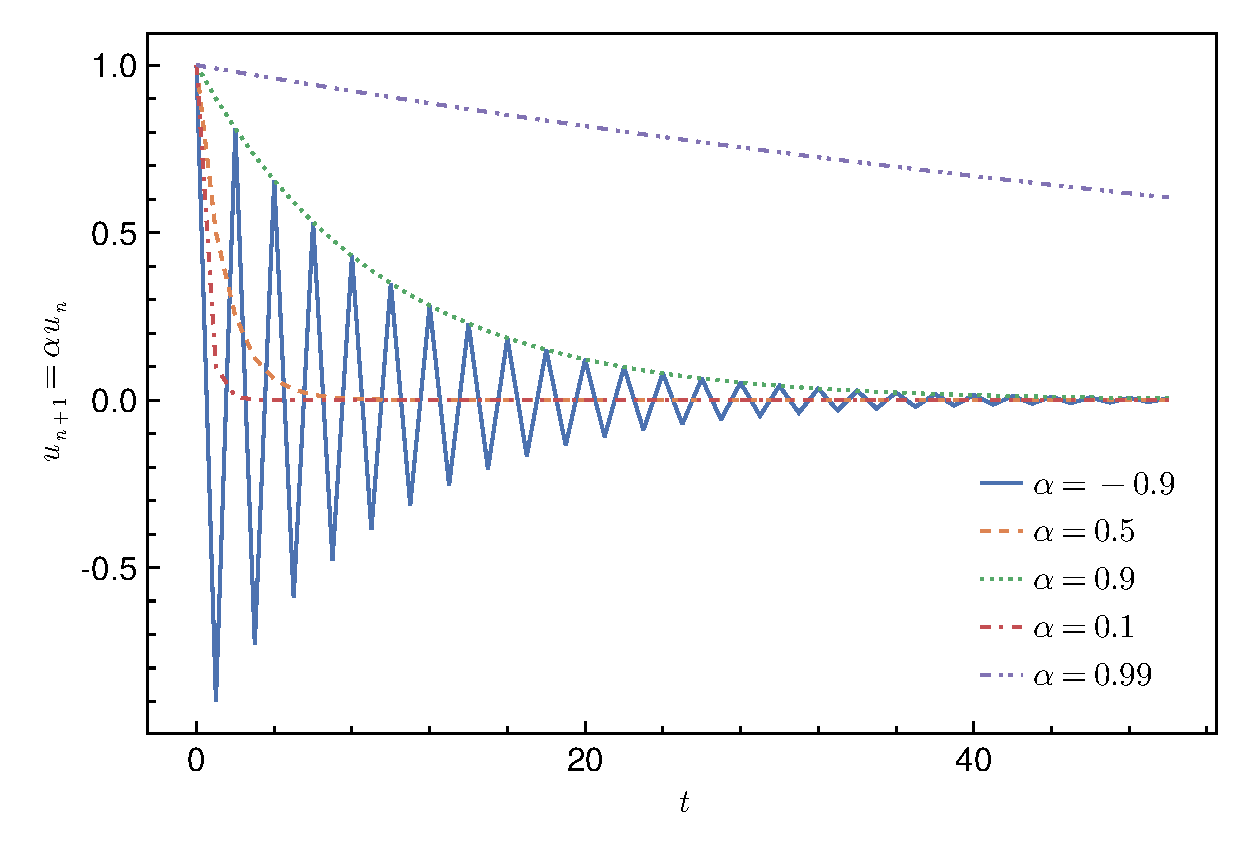
\includegraphics[width=0.5\linewidth]{images/linear_discrete_dynamical_system}
%     \caption{\textbf{Slow Convergence of Simple Linear Discrete Dynamical Systems}}
%     \label{fig:linear_discrete_dynamical_system}
% \end{figure}

\citet{rico1992discrete, bulsari1995neural} describe several other shortcomings of using discrete steady-state dynamics over continuous steady-state dynamics. These issues combined motivate changing from a discrete description of the system (the fixed point or Broyden's method approach) to a continuous description of the system that allows adaptivity to change the stepping behavior and accelerate convergence.

To this end, we propose an alternate formulation for DEQs by modeling a continuous dynamical system (Continuous DEQ) where the forward pass is represented by an ODE which is solved from $t_0 = 0$ to $t_1 = \infty$:
%
\begin{equation}
    \frac{dz}{dt} = \func{f_\theta}{z, x} - z
\end{equation}
%
where $f_\theta$ is an explicit neural network. Continuous DEQs leverage fast adaptive ODE solvers, which terminate automatically once the solution is close to a steady state, i.e., $\frac{dz^*}{dt} = 0$, which then satisfies $\func{f_\theta}{z^*, x} = z^*$ and is thus the solution to the same implicit system as before.

The Continuous DEQ can be considered an infinite-time neural ODE in this form. However, almost paradoxically, the infinite time version is cheaper to train than the finite time version as its solution is the solution to the nonlinear system, meaning the same implicit differentiation formula of the original DEQ holds for the derivative. This means that no backpropagation through the steps is required for the Continuous DEQ, and only a linear system must be solved. In \Cref{sec:experiments}, we empirically demonstrate that Continuous DEQs outperform Neural ODEs in terms of training time while achieving similar accuracies.

% Indeed, the robustness of the DEQ is even improved through this process because, in practice, the maximum iterations of the DEQ are bound~\citep{bai_deep_2019, bai_multiscale_2020, bai2021stabilizing}. DEQs often do not converge to a steady state due to this bound. In \Cref{sec:experiments}, we observe that for small-scale problems Skip~DEQs improve convergence to steady state  even where a DEQ fails due to its increased convergence speed. However, this behavior fades away once we move to the higher parameter count regime. When combining Skip~DEQs % This ability allows Skip DEQs to be trained with a more stable gradient signal since the adjoint equation assumes steady-state convergence during the forward pass.

\section{Skip Deep Equilibrium Networks}
\label{sec:skip_deqs}

\citet{bai_deep_2019, bai_multiscale_2020} set the initial condition $u_0 = 0$ while solving a DEQ. Assuming the existence of a steady state, the solvers will converge given enough iterations. However, each iteration is expensive, and a poor guess of the initial condition makes the convergence slower. To counteract these issues, we introduce an alternate architecture for DEQ (Skip~DEQ), where we use an explicit model $g_\phi$ to predict the initial condition for the steady-state problem $u_0 = g_\phi(x)$\footnote{We note that the concurrent work \citet{bai2021neural} introduced a similar formulation as a part of HyperDEQ}. We jointly optimize for $\left\{\theta, \phi\right\}$ by adding an auxiliary loss function:
%
\begin{equation}
    \mathcal{L}_{\texttt{skip}} = \lambda_{\texttt{skip}} \cdot \| f_\theta(z^*, x) - g_\phi(x) \|
\end{equation}
%
Intuitively, our explicit model $g_\phi$ better predicts a value closer to the steady-state (over the training iterations), and hence we need to perform fewer iterations during the forward pass. Given that its prediction is relatively free compared to the cost of the DEQ, this technique could decrease the cost of the DEQ by reducing the total number of iterations required. However, this prediction-correction approach still uses the result of the DEQ for its final predictions and thus should achieve robustness properties equal.

\section{Skip Regularized DEQ: Regularization Scheme without Extra Parameters}
\label{sec:skip_reg_deq}

One of the primary benefits of DEQs is the low memory footprint of these models. Introducing an explicit model $g_\phi$ increases the memory requirements for training. To alleviate this problem, we propose a regularization term to minimize the L1 distance between the first prediction of $f_\theta$ and the steady-state solution:
%
\begin{align}
    \mathcal{L}_{\texttt{skip\_reg}} = \lambda_{\texttt{skip}} \cdot \| f_\theta(z^*, x) - f_\theta(0, x) \|
\end{align}
%
This technique follows the same principle as the Skip DEQ where the DEQ's internal neural network is now treated as the prediction model. We hypothesize that this introduces an inductive bias in the model to learn simpler training dynamics.
